% Created 2015-03-17 Tue 07:17
              \documentclass{beamer}[14pt, presentation]
\institute{{  Skolkovo Institute of Science and Technology \vskip 6mm  Institute of Numerical Mathematics, Russian Academy of Sciences}}
\usepackage{tikz,pgfplots}
\pgfplotsset{compat=1.8}
\usetikzlibrary{calc,patterns,decorations.pathreplacing,decorations.markings,decorations.pathmorphing}
\usepackage{mypgf}
\usetheme{boxes}
\usepackage{mathtools}
\usepackage{graphicx}
\usepackage{amsfonts}
\usepackage{color}
\usepackage{algorithmic} \usepackage[ruled]{algorithm}
\usepackage{concrete}
\usepackage{relsize}
\usepackage{accents}
\usepackage{tikz}
\usetikzlibrary{positioning,fit,shapes,arrows}
\usepackage[version=3]{mhchem} %For the chemical formulas
\usepackage[resetlabels]{multibib}
\setbeamertemplate{bibliography entry title}{}
\setbeamertemplate{bibliography entry location}{}
\setbeamertemplate{bibliography entry note}{}
\setbeamertemplate{bibliography item}{\insertbiblabel}
\newcites{prep}{A}
\newcites{pub}{B}
\newcites{talks}{C}
\newcites{sems}{C}
\centering
\def\A{\mathbf{A}}
\def\V{\mathbf{V}}
\def\B{\mathbf{B}}
\def\C{\mathbf{C}}
\def\rank{\mathop{\mathrm{rank}}\nolimits}
\def\reshap{\mathrm{reshape}}
\DeclareMathOperator*{\RP}{\Join}
\DeclareMathOperator*{\TProd}{\otimes}
\newcommand{\CoreInd}[2]{#1_{#2}}
\newcommand*{\dt}[1]{\accentset{\mbox{\large\bfseries .}}{#1}}
\def\calM{\mathcal{M}}
\def\calR{\mathcal{R}}
\input{../pictures/pics/include.tex}
\newcommand{\SumMultInd}[2]{\sum_{\MultInd{#1}\in\MultIndSet{#2}}}
\newcommand{\IProd}[2]{\left\langle#1,#2\right\rangle}
\newcommand{\MConj}[1]{{#1}^{\ast}}
\newcommand{\MTran}[1]{{#1}^{\top}}
\newcommand{\MInv}[1]{{#1}^{-1}}
\newcommand{\SpMin}[1]{\boldsymbol{\lambda_{\min}}\left(#1\right)}
\newcommand{\SpMax}[1]{\boldsymbol{\lambda_{\max}}\left(#1\right)}
\DeclareMathOperator{\Rank}{rank}
\DeclareMathOperator{\Cond}{cond}
\DeclareMathOperator{\Diag}{diag}
\DeclareMathOperator{\Tridiag}{tridiag}
\DeclareMathOperator{\Span}{span}
\newcommand{\DiscrRange}[2]{#1,\ldots,#2}
\newcommand{\InDiscrRange}[2]{=\DiscrRange{#1}{#2}}
\newcommand{\NotInDiscrRange}[2]{\ne\DiscrRange{#1}{#2}}
\newcommand{\DiscrRangeSet}[2]{\Set{#1, \ldots ,#2}}
\newcommand{\InDiscrRangeSet}[2]{\in\DiscrRangeSet{#1}{#2}}
\newcommand{\NotInDiscrRangeSet}[2]{\notin\DiscrRangeSet{#1}{#2}}
\newcommand{\ContRange}[2]{\left[#1,#2\right]}
\newcommand{\InContRange}[2]{\in\ContRange{#1}{#2}}
\newcommand{\Par}[1]{\left(#1\right)}
\newcommand{\SqBr}[1]{\left[#1\right]}
\newcommand{\CuBr}[1]{\left\{#1\right\}}
\newcommand{\Set}[1]{\left\{#1\right\}}
\newcommand{\Vector}[1]{#1}
\newcommand{\Tensor}[1]{#1}
\newcommand{\VEl}[1]{{}_{#1}}
\newcommand{\MEl}[2]{{}_{\substack{#1 \\ #2}}}
\newcommand{\CEl}[2]{{}_{#1}}
\newcommand{\TenInd}[2]{#1_{#2}}
\newcommand{\VecIndEl}[3]{#1_{#2\;}{}_{\substack{\\[2pt] #3}}}
\newcommand{\MatrIndEl}[4]{#1_{#2\;}{}_{\substack{\\[2pt] #3 \\ #4}}}
\newcommand{\CoreIndEl}[3]{#1_{#2}\Par{#3}}
\newcommand{\El}[1]{\Par{#1}}
\newcommand{\Core}[1]{#1}
\newcommand{\ElTensor}[2]{\Tensor{#1}\left(#2\right)}
\newcommand{\ElCP}[3]{\Core{#1}\left(#3,#2\right)}
\newcommand{\ElTT}[4]{\Core{#1}\left(#2,#4,#3\right)}
\newcommand{\EllTT}[3]{\Core{#1}\left(#3,#2\right)}
\newcommand{\ElrTT}[3]{\Core{#1}\left(#2,#3\right)}
\newcommand{\Kron}[2]{\KronSym\left(#1,#2\right)}
\newcommand{\NullBlock}{}
\newcommand{\VoidBlock}{\phantom{I}}
\newcommand{\Block}[2]{#1_{#2}}
\newcommand{\SubBlock}[3]{#1^{(#2)}_{#3}}
\newcommand{\Tenkm}[3]{\Tensor{#1}^{#2}_{#3}}
\newcommand{\Tenm}[2]{\Tensor{#1}_{#2}}
\newcommand{\TenPk}[2]{\Tensor{#1}^{(#2)}}
\newcommand{\TenPkm}[3]{\Tensor{#1}^{(#2)}_{#3}}
\newcommand{\TenBk}[2]{\Tensor{#1}^{[#2]}}
\newcommand{\TenBkm}[3]{\Tensor{#1}^{[#2]}_{#3}}
\newcommand{\Vecm}[2]{\Vector{#1}_{#2}}
\newcommand{\VecPk}[2]{\Tensor{#1}^{(#2)}}
\newcommand{\VecPkm}[3]{\Tensor{#1}^{(#2)}_{#3}}
\newcommand{\VecBk}[2]{\Tensor{#1}^{[#2]}}
\newcommand{\VecBkm}[3]{\Tensor{#1}^{[#2]}_{#3}}
\newcommand{\MatrixWTT}{\mathcal{W}}
\newcommand{\FiltersWTT}{\mathcal{F}}
\setbeamertemplate{navigation symbols}{}
\usepackage{polyglossia}   %% загружает пакет многоязыковой вёрстки
\setdefaultlanguage{english}  %% устанавливает главный язык документа
\defaultfontfeatures{Ligatures=TeX,Mapping=tex-text,Scale=1.2}  %% свойства шрифтов по умолчанию
\setmainfont[Ligatures={TeX,Historic}]{Minion Pro} %% задаёт основной шрифт документа
\setsansfont{Minion Pro}                    %% задаёт шрифт без засечек
\setmonofont{Minion Pro}               %% задаёт моноширинный шрифт
%\newfontfamily\humor{Humor Sans}
\let\acute\relax
\let\grave\relax
\let\ddot\relax
\let\tilde\relax
\let\bar\relax
\let\breve\relax
\let\check\relax
\let\hat\relax
\let\dot\relax
\let\mathring\relax
\usepackage{skoltech}
\usetheme{default}
\author{I. V. Oseledets}
\date{17 March 2015}
\title{Low-rank approximation of matrices \& tensor with application to dynamical and optimization problems}
\hypersetup{
  pdfkeywords={},
  pdfsubject={},
  pdfcreator={Emacs 24.3.50.2 (Org mode 8.2.3c)}}
\begin{document}

\maketitle
\section{Motivation}
\label{sec-1}
\begin{frame}[label=sec-1-1]{Main points}
I will talk about numerics in high dimensions
\begin{itemize}
\item High-dimensional problems are hard (\alert{curse of dimensionality}) \pause
\item Fascinating algorithms appear in applications \pause
\item Generally do not become a universal computational tool
(problem-dependent)
\end{itemize}

Our goal is to create a universal set of tools for high-dimensional problems!
\end{frame}

\begin{frame}[label=sec-1-2]{Tensor}
\begin{itemize}
\item Matrix is  a \alert{two-dimensional array}
\item Tensor is   a $d$-dimensional array, $A(i_1,\ldots,i_d)$
\end{itemize}
\vskip 2mm
\begin{small}
Suddenly everything is much more complicated for tensors!
\end{small}

\includegraphics[height=0.4\textheight]{../pictures/cube.png}
\end{frame}

\begin{frame}[label=sec-1-3]{Important ``tensor'' people (not all!)}
\begin{columns}
\begin{column}{0.25\textwidth}
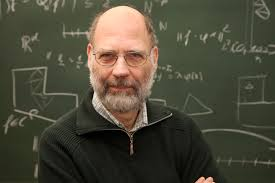
\includegraphics[height=0.15\textheight]{hackbusch.jpeg}
\vskip 2mm
{\small W. Hackbusch}
\vskip 2mm
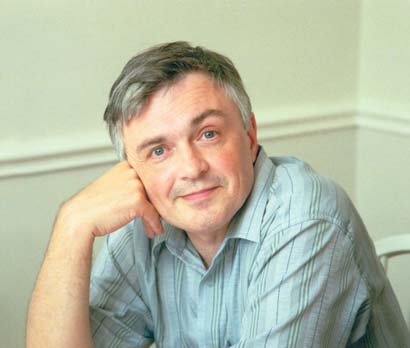
\includegraphics[height=0.15\textheight]{tee1.jpg}
\vskip 2mm
{\footnotesize E. Tyrtyshnikov}
\vskip 2mm
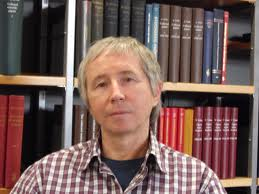
\includegraphics[height=0.15\textheight]{khor.jpeg}
\vskip 2mm
{\footnotesize B. Khoromskij}
\end{column}

\begin{column}{0.25\textwidth}
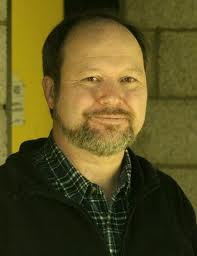
\includegraphics[height=0.15\textheight]{schneider.jpeg}
\vskip 2mm
{\footnotesize R. Schneider}
\vskip 2mm
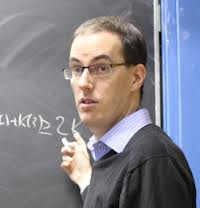
\includegraphics[height=0.15\textheight]{grasedyck.jpeg}
\vskip 2mm
{\footnotesize L. Grasedyck}
\vskip 2mm
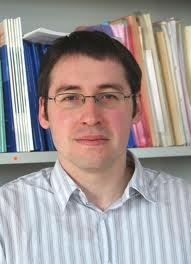
\includegraphics[height=0.15\textheight]{kressner.jpeg}
\vskip 2mm
{\footnotesize D. Kressner}
\end{column}

\begin{column}{0.25\textwidth}
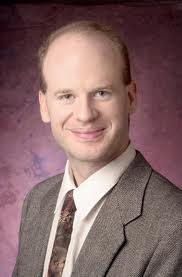
\includegraphics[height=0.15\textheight]{Mohlenkamp.jpeg}
\vskip 2mm
{\footnotesize M. Mohlenkamp}
\vskip 2mm
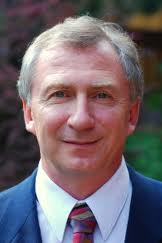
\includegraphics[height=0.15\textheight]{beylkin.jpeg}
\vskip 2mm
{\footnotesize G. Beylkin}
\vskip 2mm
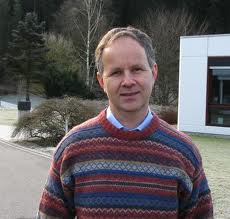
\includegraphics[height=0.15\textheight]{lubich.jpeg}
\vskip 2mm
{\footnotesize C. Lubich}
\end{column}

\begin{column}{0.25\textwidth}
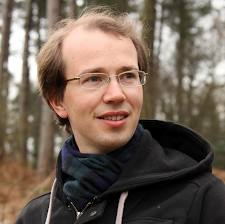
\includegraphics[height=0.15\textheight]{drraug.jpeg}
\vskip 2mm
{\footnotesize D. Savostyanov}
\vskip 2mm

\includegraphics[height=0.15\textheight]{dolgov.jpeg}
\vskip 2mm
{\footnotesize S. Dolgov}
\vskip 2mm
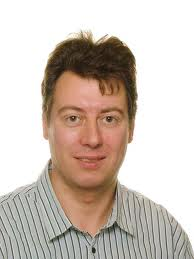
\includegraphics[height=0.15\textheight]{lathauwer.jpeg}
\vskip 2mm
{\footnotesize L. De Lathauwer}
\end{column}
\end{columns}
\end{frame}
\begin{frame}[label=sec-1-4]{Reviews}
Now there are several books / reviews: 

\begin{itemize}
\item T. Kolda, B. Bader ``Tensor decompositions and applications'', SIREV
2009 -- outdated
\item B. N. Khoromskij,
\end{itemize}
Tensors-structured Numerical Methods in Scientific Computing: Survey
on Recent Advances (2010)
\begin{itemize}
\item L. Grasedyck, D. Kressner, C. Tobler, A literature survey of
low-rank tensor approximation techniques (2013)
\item W. Hackbusch, Tensor spaces and numerical tensor calculus, Springer, 2012.
\end{itemize}
\end{frame}

\section{Our story}
\label{sec-2}
\begin{frame}[label=sec-2-1]{Motivation}
\begin{onlyenv}<1>
\alert{Main point}
\begin{itemize}
\item High-dimensional problems appear in many applications
\item Standard methods do not scale well with $d$
\end{itemize}
\end{onlyenv}

\begin{onlyenv}<2>
Solving differential / integral equations on fine grids
  \vskip 2mm
 Typical cost: \alert{$\mathcal{O}(N^3)$} $\rightarrow$
  \alert{$\mathcal{O}(N)$} or \alert{$\mathcal{O}(\log^{\alpha} N)$}.
\includegraphics[width=0.8\linewidth]{../pictures/3d_lshape_light.pdf}
\end{onlyenv}

\begin{onlyenv}<3>
Ab initio computations and computational material design
\begin{columns}
\begin{column}{0.45\linewidth}
Protein-ligand docking
\includegraphics[width=\linewidth]{../pictures/protein-ligand.pdf}
\end{column}
\begin{column}{0.45\linewidth}
Solving the Hartree-Fock equation (great progress: V. Khoromskaya, B. Khoromskij; the picture is from our HF-solver)
    \resizebox{\textwidth}{!}{\includegraphics{../pictures/ethanol-eps-converted-to.pdf}}
\end{column}
\end{columns}
\end{onlyenv}
\begin{onlyenv}<4>
Model reduction
\begin{columns}
\begin{column}{0.45\linewidth}
\includegraphics[width=\linewidth]{../pictures/circles2.pdf}
\end{column}
\begin{column}{0.45\linewidth}
\alert{Diffusion equation (Kressner, Tobler)} 
\vskip 2mm
$\nabla a(p) \Delta u = f(p)$, \\
$p = (p_1,p_2,p_3,p_4)$ \\
Approximate $u$ from few snapshots.
\end{column}
\end{columns}
\end{onlyenv}
\begin{onlyenv}<5>
Data compression and mining
\begin{columns}
\begin{column}{0.45\linewidth}
Картинки
\includegraphics[width=\linewidth]{../pictures/lena512_90.pdf}
\end{column}
\begin{column}{0.45\linewidth}
Computational data compression
\includegraphics[width=\linewidth]{../pictures/ocean.png}
\end{column}
\end{columns}
\end{onlyenv}
\end{frame}
\begin{frame}[label=sec-2-2]{An ad}
 \begin{small}
Biological modelling:  \\ 
V. Kazeev, M. Khammash, M. Nip., C. Schwab 
 \vskip 2mm
 \end{small}
\includegraphics[width=.9\linewidth]{../pictures/graphsColor/cycle.pdf}

\begin{itemize}
\item tensor method: $10^3 - 10^4$ on a notebook in  MATLAB
\item 1500 cores, Monte-Carlo: $10^5$-sec
\end{itemize}
\end{frame}
\begin{frame}[label=sec-2-3]{Main problem}
\alert{We need to approximate high-dimensional tensors}
\end{frame}

\begin{frame}[label=sec-2-4]{Separation of variables}
One of the few fruitful ideas is \alert{separation of variables} \vskip 2mm
Main task: \alert{how to do it numerically?}
\end{frame}

\begin{frame}[label=sec-2-5]{Canonical format}
Starting point: \alert{CP-format} \vskip 2mm
$A(i_1,\ldots,i_d) = \sum_{\alpha=1}^r U_1(i_1,\alpha) \ldots U_d(i_d,
\alpha)$
\vskip 2mm
\alert{No robust algorithms}: best approximation with fixed rank may
not exist!
\end{frame}

\begin{frame}[label=sec-2-6]{Everything is good in 2D}
2D: $A = UV^{\top}$, we have the Singular Value Decomposition \vskip
2mm
We want the methods of such quality in many dimensions!
\end{frame}

\begin{frame}[label=sec-2-7]{TT \& HT formats}
Independently, in 2009 two formats were proposed: 
\begin{itemize}
\item Tree-Tucker (O. \& Tyrtyshnikov) became the Tensor Train;
\item HT-format (Hackbusch, Kuhn, Grasedyck).
\end{itemize}
Both are based on the hierarchical separation of indices
\vskip 2mm
\end{frame}

\begin{frame}[label=sec-2-8]{TT-format}
$A(i_1,\ldots,i_d) = G_1(i_1) G_2(i_2) \ldots G_d(i_d)$, \vskip 2mm
where $G_k(i_k)$ --- matrix of size $r_{k-1} \times r_k$.
\end{frame}

\section{One more story}
\label{sec-3}
\begin{frame}[label=sec-3-1]{Tensor networks, MPS(1)}
Other areas: \vskip 2mm
TT is Matrix product states 
\vskip 2mm (Used to represent spin wavefunctions)
\vskip 2mm
$H \psi = E \psi$ \vskip 2mm
$\psi = \psi(S_1, \ldots, S_N)$ --- spin system \vskip 2mm
Algorithms  (Wilson renormalization group, Density Matrix
Renormalization Group) were proposed a lot earlier.  \\
Vidal, Cirac, Verstraete, \ldots
\vskip 2mm
Brought to mathematics by T. Huckle and R. Schneider
\end{frame}

\begin{frame}[label=sec-3-2]{Tensor networks, MPS(2)}
DMRG, MPS,  tensor networks: \vskip 2mm
Big community, brilliant algorithms for eigenvalues / time-dependent
problems / eigenvalue problems
\end{frame}

\section{One more story}
\label{sec-4}
\begin{frame}[label=sec-4-1]{Markov random fields}
Markov random fields (wiki picture) \\
\includegraphics[height=0.4\textheight]{../pictures/Markov_random_field_example.png}
Edge corresponds to a function $\psi_{AD}$, 
\vskip 2mm
$p(A, B, C, D, E) = \psi_{AD} \psi_{AB} \psi_{DE} \psi_{CE}$ \vskip 2mm
Algorithm: \alert{belief propagation for trees!}
\end{frame}

\begin{frame}[label=sec-4-2]{Recent successes}
Linear tree $\rightarrow$ \alert{hidden markov models}
\vskip 2mm
Spectral methods for learning HMM (Hsu, Kakade, 2009) are based on the
singular value decomposition
\end{frame}

\section{TT-format}
\label{sec-5}
\begin{frame}[label=sec-5-1]{Definition}
Tensor is said  in the TT-format, if 
\vskip 2mm
$A(i_1,\ldots,i_d) = G_1(i_1)G_2(i_2) \ldots G_d(i_d)$,
\vskip 2mm
where $G_k(i_k)$ --- matrix of size $r_{k-1} \times r_k$, $r_0 = r_d = 1$
\\
$r_k$ are called \alert{TT-ranks} \\
$G_k(i_k)$ (which are $r_{k-1} \times n_k \times r_k$ tensors)
are called  \alert{cores}
\end{frame}

\begin{frame}[label=sec-5-2]{TT in a nutshell}
\begin{itemize}
\item $\mathbf{A}$ --- canonical rank $r$ $\rightarrow$ $r_k \leq r$
\item TT-ranks are matrix ranks, \textcolor{purple}{TT-SVD}
\item All arithmetic, linear in $d$, polynomial in $r$
\item Fast \textcolor{purple}{\sc tensor rounding}
\item TT-cross, \textcolor{purple}{exact interpolation formula}, recent:
quasioptimality results (D. Savostyanov)
\item Q(Quantics, Quantized)-TT decomposition --- binarization (or
tensorization) of vectors and matrices (B. Khoromskij, O.)
\item TT-Toolbox -- software, S. V. Dolgov, I.V. Oseledets,
D. V. Savostyanov, V. A. Kazeev
\end{itemize}
\end{frame}

\begin{frame}[label=sec-5-3]{TT-ranks --- matrix ranks}
\begin{onlyenv}<1-2>
Define unfoldings: \\
 $A_k = A(i_1 \ldots i_k; i_{k+1} \ldots i_d)$, $n^k \times n^{d-k}$
matrix
\end{onlyenv}

\begin{onlyenv}<2>
Theorem: There exists a TT-decomposition with TT-ranks
$$r_k = \rank A_k$$
\end{onlyenv}

\begin{onlyenv}<3>
The proof is constructive and gives the TT-SVD algorithm (Vidal
algorithm in quantum information)
\end{onlyenv}

\begin{onlyenv}<4>
There is no exact low ranks need stability estimate! \\
\begin{theorem}[Approximation theorem]
If $A_k = R_k + E_k$, $||E_k|| = \varepsilon_k$
$$||\mathbf{A}-\mathbf{TT}||_F \leq \sqrt{\sum_{k=1}^{d-1} \varepsilon^2_k}.$$
\end{theorem}
\end{onlyenv}
\end{frame}
\begin{frame}[label=sec-5-4]{Fast linear algebra}
\begin{onlyenv}<1>
Addition, Hadamard product, scalar product \\
 All linear in $d$ \\
\end{onlyenv}

\begin{onlyenv}<2>
$C(i_1,\ldots,i_d) = A(i_1,\ldots,i_d) B(i_1,\ldots,i_d)$ \\
   $$C_k(i_k) = A_k(i_k) \otimes B_k(i_k),$$
ranks are multiplied
\end{onlyenv}
\end{frame}

\begin{frame}[label=sec-5-5]{Tensor rounding}
\begin{onlyenv}<1>
$\mathbf{A}$ is given in  TT-format with suboptimal ranks. \\
  Who to reapproximate? \\
\end{onlyenv}

\begin{onlyenv}<2>
It can be done in $\mathcal{O}(dnr^3)$ operations 
\vskip 2mm
\end{onlyenv}
\end{frame}

\begin{frame}[label=sec-5-6]{Cross approximation in d-dimensions}
\begin{onlyenv}<1-2>
What if a tensor is given as a ``black box''?
\vskip 2mm
\end{onlyenv}

\begin{onlyenv}<2>
O., Tyrtyshnikov, 2010: \\
TT-cross approximation of multidimensional arrays\\
We can exactly interpolate a rank-$r$ on
\textcolor{purple}{$\mathcal{O}(dnr^2)$} elements \vskip 2mm
$\mathcal{I}_k = (i^{(\alpha)}_1,\ldots,i^{(\alpha)}_k)$, \vskip 2mm
$\mathcal{J}_k = (i^{(\beta)}_k, \ldots,i^{(\alpha)}_d)$
\vskip 2mm
$A_k = A(\mathcal{I}_k,i_k,\mathcal{J}_{k+1})$
\end{onlyenv}
\end{frame}

\begin{frame}[label=sec-5-7]{Making everything a tensor: QTT}
\begin{onlyenv}<1>
\begin{itemize}
\item Prequel: E. E. Tyrtyshnikov (2003)
\item I. V. Oseledets (2009)
\item B. N. Khoromskij (2009)
\end{itemize}
\vskip 2mm
  ``Simple'' idea: \textcolor{purple}{to make everything a tensor} (we
  have  software, need examples)
\end{onlyenv}

\begin{onlyenv}<2>
Let $f(x)$ -- function of one variable ($f(x) = \sin x$).
\vskip 2mm
If $v$ -- vector of values on a uniform grid with  $2^d$  nodes.
\vskip 2mm
Reshape $v$ into a  $2 \times 2 \times \ldots \times 2$
$d$-dimensional tensor.
\vskip 2mm
Compute TT-decomposition!
\vskip 2mm
It is a \textcolor{purple}{QTT-format}
\end{onlyenv}

\begin{onlyenv}<3>
 If $f(x)$ is such that 
$$f(x+y) = \sum_{\alpha=1}^r u_{\alpha}(x) v_{\alpha}(y),$$
then QTT-ranks are bounded by $r$
\vskip 2mm
Conclusion: \\
\begin{itemize}
\item $f(x) = \exp(\lambda x)$
\item $f(x) = \sin (\alpha x + \beta)$
\item $f(x)$ - polynom
\item $f(x)$ - Rational function
\end{itemize}
\end{onlyenv}
\end{frame}

\begin{frame}[label=sec-5-8]{TT-Toolbox}
Software: \url{http:/github.com/oseledets/TT-Toolbox}
\begin{itemize}
\item Basic operations in TT-format
\item Advanced operations in  TT-format (linear systems, eigenvalues,
non-stationary probems, interpolation)
\item Main operators
\item Open-source
\item S. V. Dolgov, V. A. Kazeev, I. V. Oseledets, D. V. Savostyanov, \ldots{}
\end{itemize}
\end{frame}

\section{Applications and main problems}
\label{sec-6}
\begin{frame}[label=sec-6-1]{Applications and main problems(1)}
High-dimensional linear systems:
\vskip 2mm
\alert{
$Ax = f$, $x = X(i_1, \ldots, i_d)$
}
\vskip 2mm
Typical cases:
\begin{itemize}
\item High-dimensional PDE on a tensor-product grid (Chemical master
equation, Fokker-Planck equation)
\item Parametric / stochastic PDE:
\vskip 2mm
$A(p) u(p) = f(p)$, $p = (p_1, \ldots, p_m)$, 
\vskip 2mm
After discretization:  
\vskip 2mm
$u = u(i, p_1, \ldots, p_M)$ --- a tensor!
\end{itemize}
\end{frame}
\begin{frame}[label=sec-6-2]{Applications and main problems (2)}
High-dimensional eigenvalue problems:
\vskip 2mm
\alert{
$Ax = \lambda x$, $x = X(i_1, \ldots, i_d)$}
\vskip 2mm
Typical cases:
\begin{itemize}
\item Spin systems (classical case, where MPS come from)
\item Vibrational computations, $A = -\frac{1}{2} \Delta + V$
\item Parametric problems (as well).
\end{itemize}
\end{frame}
\begin{frame}[label=sec-6-3]{Applications and main problems (3)}
High-dimensional unsteady problems:
\vskip 2mm
\alert{$\frac{dy}{dt} = Ay, y = Y(i_1, \ldots, i_d)$}
\vskip 2mm
Typical cases:
\begin{itemize}
\item Chemical master equation
\item Computation of vibrational spectra
\end{itemize}
\end{frame}
\begin{frame}[label=sec-6-4]{Applications and main problems (4)}
Interpolation of multivariate functions:
\vskip 2mm
$f(x_1, \ldots, x_d)$ is given as a subroutine
\vskip 2mm
Typical cases:
\begin{itemize}
\item Global optimization problems
\item Approximation of expensive parametric dependencies
\item Many more\ldots{}
\end{itemize}
\end{frame}
\begin{frame}[label=sec-6-5]{Summary}
Several basic problems:
\begin{itemize}
\item $Ax = f$
\item $Ax = \lambda x$
\item $\frac{dy}{dt} = Ay$
\item Interpolation
\end{itemize}
The solution is sought on a low-parametric manifold: 
\vskip 2mm
General strategy:
\vskip 2mm
Reformulate as $J(x) \rightarrow \min$, minimize over a manifold.
\end{frame}

\begin{frame}[label=sec-6-6]{Summary(2)}
There are \alert{very efficient algorithms} for all type of problems!
\begin{itemize}
\item Linear systems: AMEN-solver (Dolgov, Savostyanov)
\item Eigenvalue solver: AMEN-solver, EIGB-solver (Dolgov, Savostyanov,
Oseledets, Khoromskij)
\item Nonstationary case: KSL-scheme (Oseledets, Lubich, Vanderbreycken)
\item Interpolation: AMEN-cross (Dolgov, Savostyanov, Oseledets)
\end{itemize}
\end{frame}

\section{TT-KSL scheme}
\label{sec-7}
\begin{frame}[label=sec-7-1]{Solving non-stationary problems}
Considerable interest:
\vskip 2mm
$\frac{dy}{dt} = Ay$,
\vskip 2mm
$Y = Y(i_1,\ldots,i_d)$
\vskip 2mm
By writing down the equations for the parameters on the manifold!
\vskip 2mm
We now have a \alert{very efficient integrator}: \vskip 2mm KSL-scheme
\end{frame}

\begin{frame}[label=sec-7-2]{Dynamical low-rank approximation}
 Given $A(t)$, approximate by $X(t) \in \mathcal{M}$, \vskip 2mm where
 $\mathcal{M}$ --- manifold:
 \vskip 2mm
Dirac-Frenkel principle:
\begin{equation*}
 (\dt{A} - \dt{X}, v) = 0, \quad v \in \mathcal{T}(\mathcal{M}),
\end{equation*}
$\mathcal{T}$ is the tangent space.
\vskip 2mm
\alert{Gives equations of motion}
\end{frame}

\begin{frame}[label=sec-7-3]{KSL-scheme for the TT-format}
Equation of motions have been derived:
\begin{itemize}
\item Matrix case, Tucker case: (H.-D. Meyer, C. Lubich, O. Koch)
\item TT-format, HT-format (C)
\end{itemize}
\end{frame}

\begin{frame}[label=sec-7-4]{Matrix case}
Matrix case
\vskip 2mm
\begin{footnotesize}
C. Lubich, I.V. Oseledets, A projector-splitting integrator for
dynamical low-rank approximation
\vskip 2mm
\end{footnotesize}
\end{frame}

\begin{frame}[label=sec-7-5]{Dynamical low-rank appr. of matrices}
\begin{onlyenv}<1>
The equations for $U, S, V$: \\
\begin{equation*}
\begin{split}
&\dt{U} = (I - U(t) U(t)^{\top})\dt{A}(t) V(t) S(t) ^{-1}\\
&\dt{V} = (I - V(t)V(t)^{\top})\dt{A}(t)^{\top} U(t) S(t)^{-\top} \\
&\dt{S} = U(t)^{\top} \dt{A}(t) V(t).
\end{split}
\end{equation*}
\end{onlyenv}

\begin{onlyenv}<2>
\begin{equation*}
\dt{X} = P_X(\dt A), \quad P_x(\dt A) = \dt A - ( I - UU^{\top}) \dt A( I - VV^{\top}).
\end{equation*}
No multiplication by $S^{-1}$
\end{onlyenv}
\end{frame}

\begin{frame}[label=sec-7-6]{KSL integrator}
Algorithm:
\begin{itemize}
\item K-step: $\dt{(US)} = \dt{A} V$
\item QR: $K_1 = U_1 \widehat{S}_1$
\item S-step: $\dt{S} = -U^{\top} \dt{A} V$ (backward in time!)
\item L-step: $\dt{(VS^{\top})} = \dt{A}^{\top} U$
\item QR: $L_1 = U_1 \widetilde{S}_1$
\end{itemize}
\end{frame}

\begin{frame}[label=sec-7-7]{TT-KSL integrator}
Just apply the KSL scheme recursively!
\tikzstyle{index} = [minimum size =8em, rectangle, every
 edge/.style={link}]
 \tikzstyle{lab} = [minimum width =8em, rectangle, every edge/.style={link}]
 \newsavebox{\mycircle}
\savebox{\mycircle}{
 \begin{tikzpicture}
\begin{scope}
\filldraw[fill=black, draw=black] (0,0) arc (-90-45:90-45:1) -- (0,0);  
\filldraw[fill=white, draw=black] (0,0) arc (-90-45:-270-45:1) -- (0,0);
\end{scope}
\end{tikzpicture}}
\newsavebox{\qrcirc}
\savebox{\qrcirc}{
\begin{tikzpicture}
\filldraw[fill=black,draw=black] circle(0.5);
\end{tikzpicture}}
\newsavebox{\mycir}
\savebox{\mycir}{
\begin{tikzpicture}
\filldraw[fill=black, draw=black] (0,0) arc (-90+45:90+45:1) -- (0,0);  
\filldraw[fill=white, draw=black] (0,0) arc (-90+45:-270+45:1) -- (0,0);
\end{tikzpicture}}
\newsavebox{\mysun}
\savebox{\mysun}{\begin{tikzpicture}[align=center]
\pgfmathsetmacro{\myrad}{0.5}
\begin{scope}
\filldraw[fill=white, draw=black] (0,0) circle (\myrad);
\foreach \an in {0,30,...,360} 
  \draw (\myrad*cos \an, \myrad*sin \an) -- (2*\myrad*cos \an, 2*\myrad*sin \an);
\end{scope}
\end{tikzpicture}}

 \begin{tikzpicture}
 %Variables
\pgfmathsetmacro{\mysc}{0.2}
\pgfmathsetmacro{\sepf}{2.5}
\pgfmathsetmacro{\sepT}{1}
\pgfmathsetmacro{\myh}{0.5}
 \node[lab] (A0) {Update $X_1$};
 \begin{scope}[scale=\mysc, transform shape]
 \node[index] (i01) [right = \sepT of A0]  {\usebox{\mysun}};
 \node[index] (i02) [right = \sepf of i01] {\usebox{\mycircle}};
 \node[index] (i03) [right = \sepf of i02] {\usebox{\mycircle}};
 \node[index] (i04) [right = \sepf of i03] {\usebox{\mycircle}};
 \path[-] (i01) edge (i02);
 \path[-] (i02) edge (i03);
 \path[-] (i03) edge (i04);
 \end{scope}
 \node[lab] (A1) [below= \myh of A0] {QR $\rightarrow$};
 \begin{scope}[scale=\mysc, transform shape]
 \node[index] (i11) [right = \sepT of A1]  {\usebox{\mycir}};
 \node[index] (i12) [right = \sepf of i11] {\usebox{\mycircle}};
 \node[index] (i13) [right = \sepf of i12] {\usebox{\mycircle}};
 \node[index] (i14) [right = \sepf of i13] {\usebox{\mycircle}};
 \path[draw=black] (i11) -- (i12) node[midway,index] {\usebox{\qrcirc}}; 
 \path[-] (i12) edge (i13);
 \path[-] (i13) edge (i14);
 \end{scope}
 \node[lab] (A2) [below= \myh of A1] {Update S};
 \begin{scope}[scale=\mysc, transform shape]
 \node[index] (i41) [right = \sepT of A2]  {\usebox{\mycir}};
 \node[index] (i42) [right = \sepf of i41] {\usebox{\mycircle}};
 \node[index] (i43) [right = \sepf of i42] {\usebox{\mycircle}};
 \node[index] (i44) [right = \sepf of i43] {\usebox{\mycircle}};
 \path[draw=black] (i41) -- (i42) node[midway,index,scale=0.7]{\usebox{\mysun}};
 \path[-] (i42) edge (i43);
 \path[-] (i43) edge (i44);
 \end{scope}

 \node[lab] (A3) [below= \myh of A2] {Update $X_2$};
 \begin{scope}[scale=\mysc, transform shape]
 \node[index] (i21) [right = \sepT of A3]  {\usebox{\mycir}};
 \node[index] (i22) [right = \sepf of i21] {\usebox{\mysun}};
 \node[index] (i23) [right = \sepf of i22] {\usebox{\mycircle}};
 \node[index] (i24) [right = \sepf of i23] {\usebox{\mycircle}};
 \draw (i21) -- (i22); 
 \draw (i22) -- (i23); 
 \draw (i23) -- (i24); 
 \end{scope}
\end{tikzpicture}
\end{frame}
\begin{frame}[label=sec-7-8]{KSL and MCTDH}
\begin{onlyenv}<1>
$\frac{d \psi}{dt} = i H \psi, \quad \psi(0) = \psi_0$ \vskip 2mm
$H = -\frac{1}{2} \Delta + V$, \vskip 2mm
Local problems: 
\vskip 2mm 
Small linear ODEs
\vskip 2mm
Compute $a(t) = (\psi(t), \psi(0))$ and the spectrum of $H$ from it. 
\end{onlyenv}

\begin{onlyenv}<2>
\begin{small}
            \textcolor{purple}{$ V(q_1,\ldots,q_f) = \frac{1}{2}\sum_{k=1}^f q^2_k + \lambda \sum_{k=1}^{f-1}\left(q^2_k q_{k+1} - \frac{1}{3}q^3_k \right).$}
\end{small}
\url{http://www.pci.uni-heidelberg.de/cms/mctdh.html}  
\includegraphics[width=.9\linewidth]{../pictures/mctdh-ksl-comp.pdf}
\end{onlyenv}
\end{frame}
\section{Data compression}
\label{sec-8}
\begin{frame}[label=sec-8-1]{Relation to wavelets}
The idea of QTT has a deep connection to \alert{wavelets}
\begin{itemize}
\item I. V. Oseledets, E. E. Tyrtyshnikov, Algebraic wavelet transform via
quantics tensor train decomposition
\item V. A. Kazeev,  Oseledets, I. V. , The tensor structure of a class of
adaptive algebraic wavelet transforms
\item Boris N. Khoromskij,  Sentao Miao, Superfast Wavelet Transform Using QTT Approximation. I: Haar Wavelets
\end{itemize}



You can use \alert{WTT} as a general compression technique!
\end{frame}

\begin{frame}[label=sec-8-2]{Ocean temperature}
\begin{onlyenv}<1>
The temperature (4-d array), computed using the INM-RAS global
circulation model \\
Array of size $360 \times 337 \times 40 \times 648$ --- 12 Gb.
\includegraphics[height=0.6\linewidth]{../pictures/ocean.png}
\end{onlyenv}

\begin{onlyenv}<2>
\begin{table}[H]
\begin{small}
 \begin{center}
  \begin{tabular}{cccc}
   Memory & Abs err & Rel err & Comp time\\
   497 MB & 0.0392 & 0.0004 & $\approx 500$ sec \\
   277 MB & 0.0984  & 0.0009 & $\approx 500$ sec \\
  \end{tabular}
 \caption{WTT decomposition compression}
 \end{center}
\end{small}
\end{table}
\end{onlyenv}
\end{frame}
\section{Latent variable models}
\label{sec-9}
\begin{frame}[label=sec-9-1]{Latent variable models}
\begin{onlyenv}<1-3>
Interesting applications
 \vskip 2mm 
 \alert{latent variable models}
\end{onlyenv}

\begin{onlyenv}<2-3>
Observe $S_1,\ldots,S_N$ (stock prices) 
\vskip 2mm
And here are the hidden variables
\end{onlyenv}

\begin{onlyenv}
$p(x_1,x_2) = \sum_{\alpha=1}^r p_1(x_1,h) w(h) p_2(x_2,h)$
\vskip 2mm 
 You can use tensors! (Ishteva, Le Song, Georgia Tech.)
\end{onlyenv}

\begin{onlyenv}<4>
Recovering the tree
\vskip 3mm
(M. Ishteva, Le Song)
\includegraphics[width=.9\linewidth]{../pictures/ishteva-pic.pdf}
\end{onlyenv}
\end{frame}
\section{Global optimization}
\label{sec-10}
\begin{frame}[label=sec-10-1]{Global optimization}
\begin{onlyenv}<1>
Can we apply it to the global optimization problems?
\vskip 2mm
 $f(x_1, \ldots, x_d) \rightarrow \min$
\vskip 2mm
``Naive'' idea:
\begin{enumerate}
\item Approximate $f$ by low rank
\item Find maximum, for example, by $\min (Dx, x) \rightarrow \min$
\end{enumerate}

What if \alert{no approximation exists?}
\end{onlyenv}

\begin{onlyenv}<2-3>
The cross approximation method has a potential to find maximal
absolute value!
\end{onlyenv}

\begin{onlyenv}<3>
\begin{theorem}{}
   Let $A$ be an $n \times m$ matrix, $\widehat{A}$ is an $r \times r$
   submatrix with maximal volume, then
   $$
       ||\widehat{A}||_C \geq \frac{ ||A||_C}{r^2 + r}. 
   $$
\end{theorem}
\end{onlyenv}
\begin{onlyenv}<4>
To force to the global minimum, we do shifts and transforms:
\begin{equation*}
   \widetilde{f} = \mathrm{arcctg}(f - f^* ),
\end{equation*}
where $f^*$ is the current record. 
\vskip 2mm
\alert\{Just run the standard dD-cross method, and compute maximal over all
the samples!\}
\end{onlyenv}
\end{frame}
\begin{frame}[label=sec-10-2]{Conclusions}
\begin{itemize}
\item Numerical algorithms are developing at fast rate
\item High potential impact in many applications (biology, optimization, chemistry)
\item Theory is trailing behind
\end{itemize}
\end{frame}

\begin{frame}[label=sec-10-3]{Software}
 Papers and codes: 
\begin{large}
\begin{itemize} 
\item My webpage: \textcolor{purple}{http://spring.inm.ras.ru/osel}
\item Publications: \textcolor{purple}{http://pub.inm.ras.ru}
\item TT-Toolbox
\textcolor{purple}{http://github.com/oseledets/TT-Toolbox},  \textcolor{purple}{http://github.com/oseledets/ttpy}
\end{itemize}
\end{large}
\end{frame}
% Emacs 24.3.50.2 (Org mode 8.2.3c)
\end{document}